% !TEX root = bipartite.tex

\section{Characteristics of user-object networks} \label{sec:ubnetworks}

A user-object network can be represented as a graph $G = (U, O, E)$, where $U$
is the users set, $O$ is the objects set and $E \subseteq (U \times O)$ is the
set of edges between users and objects. We denote by $n_u = |U|$ and $n_o = |O|$
the number of users and the number of objects, respectively. We denote by $m =
|E|$ the number of links or edges in the bipartite network. We define $\langle
k_U \rangle$ ($\langle k_O \rangle$) as the average degree of users (objects)
and the density of the network as $\delta(G) = \frac{m}{n_o n_u}$.

In user object networks interactions between the two types of nodes, $U$ and
$O$, are event-driven, occurring continuously, and often the same edge is
reinforced multiple times. This reinforcement can be represented as a weight
assigned to the edge between the two interacting nodes. On the other side, in
most bipartite networks there is only one interaction between two nodes (an
actor can only play once in a movie).

The behaviour of nodes is also particular. Users are active while objects are
passive. This is similar to author-paper networks but different than other
bipartite networks such as human sexual networks where both nodes are active
\citep{shang10empirical}.

\begin{figure}[t]
\centering
  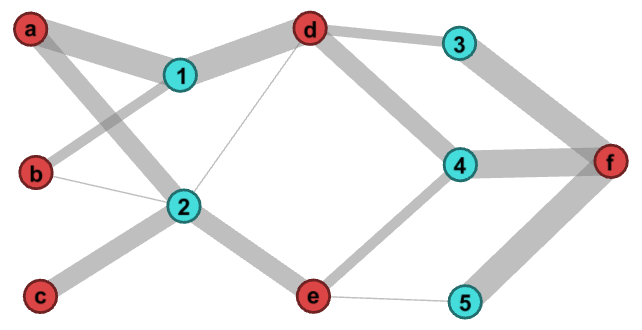
\includegraphics[width=8cm]{./figures/example_weighted.png}  
  \caption{Example of weighted bipartite network where users (blue nodes) are
  connected with objects (red nodes).
  }
\label{fig:example}
\end{figure}

Figure \ref{fig:example} illustrates a small example of a weighted bipartite
network where five users (blue nodes) are interacting with six objects (red
nodes). Thickness of an edge shows how strong the interaction is between the
user and the object (i.e. how often the user `touches` the object). The degree
of an user $u \in U$, denoted by $d(u)$, represents the number of objects
connected to that user. Similarly, the degree of an object $o \in O$, denoted by
$d(o)$, is the number of users interacting with that object. In our example,
user $1$ interacts with three objects $a$, $b$ and $d$ (has a degree of three).
Out of these, objects $a$ and $b$ are local as they are only connected to two
users ($1$ and $2$), while object $d$ reaches most of the network by being
connected to four out of a total of five users. Therefore objects $a$ and $b$
are more relevant to particular interests of user $1$ than object $d$.

\paragraph{Data}

We are using five real-world data sets and look at the characteristics of the
related user-object networks such as basic statistics, degree distributions and
clustering. The first one is a subset of the Last.fm Million Song Dataset
\citep{Bertin-Mahieux2011}, where users are connected to tags, with an edge
defined between an user and a tag if that user assigned the tag to an artist.

The second dataset was extracted from Twitter and includes tweets related to US
Politics, covering the period 01/01/2012 - 19/01/2012. This is a subset of a
bigger dataset including the US Presidential Campaign and Elections during
2012. The users in the data are the Presidential candidates, governors,
senators, political organisations, and journalists. The objects are the web
domains included in their tweets. An edge is formed between an user and a domain
if the domain was tweeted by that particular user.

The third dataset is a subset of a bigger database published by
Audioscrobbler.com containing information about users and the music they
listened. In the network representation, an user is connected to an artist
with edges weighted based on how often they listen songs from that artist. The
Movielens dataset includes ratings (from 1 to 5) of movies by 2000 users,
represented as a network. For the purpose of this paper only edges with ratings 4 and 5
were considered (movies that users actually liked). Finally, the last dataset
comes from the popular social bookmarking web site delicious.com and includes
the network of 973 users and the tags they used for bookmarking.

\begin{table}[!h] \centering
\begin{tabular}{ l | c c c c c c }
 Data & $n_u$ & $n_o$ & $m$ & $\langle k_U \rangle$ & $\langle k_O \rangle$ &
 $\delta(G)$ \\
\hline
Last.fm & 1,892 & 9,748 & 35,813 & 18 & 3 & 0.19\% \\
Twitter & 1,842 & 3,744 & 13,864 & 7 & 3 & 0.2\% \\
Audioscrobbler & 183 & 21,443 & 39,195 & 214 & 1 & 1\% \\
Movielens & 2,000 & 3,336 & 192,922 & 96 & 57 & 2.9\% \\
Delicious & 973 & 28,695 & 126,007 & 129 & 4 & 0.45\% \\
\end{tabular}
\caption{Statistics of the five real-world datasets.}
\label{tab:datasets}
\end{table}

The basic statistics for these networks are presented in Table
\ref{tab:datasets}. All networks have relatively low density (they are sparse),
between 0.19\% and 2.9\%. This is important because it allows for optimization
of clustering and community detection algorithms. As we will see below this is
not the case for the projections of these bipartite networks.

\paragraph{Projection}

Due to the shortage in tools and notions available for two-mode networks a
common approach is to transform such network into its projection by using one
of its sets of nodes as a base. For example one can project the network on the
users $U$ (objects $O$) by setting a (weighted) edge between two users (objects)
that have at least one object (user) in common. Based on the number of common
objects (users), weights can be assigned to edges in the projected network. We
define the users-projected network as $G_U = (U, E_U)$ and objects-projected
network as $G_O = (O, E_O)$. The number of edges is $m_U = |E_U|$ and $m_O =
|E_O|$, respectively. The density of the projected networks is $\delta(G_U) =
\frac{2 m_U}{n_u (n_u-1)}$ and $\delta(G_O) = \frac{2 m_O}{n_o (n_o-1)}$,
respectively.

One of the unwanted effects of projection is an inflation of the number of links
in the resulted network \citep{latapy2008basic}, which can be noticed in random
networks as well. \citet{newman2001random} have shown that projecting a random
bipartite graph can result in very dense networks with high clustering
coefficient. In the real world case these dense networks are limiting the
computations that could be performed to extract properties and detect community
structure. 

\begin{table}[!h] \centering
\begin{tabular}{ l | c c c c }
Data & $m_U$ & $m_O$ & $\delta(G_U)$ & $\delta(G_O)$ \\
\hline
Last.fm & 686,536 & 322,226 & 38.3\% & 0.6\% \\
Twitter & 446,892 & 88,044 & 26.3\% & 1.2\% \\
Audioscrobbler & 10,453 & 11,253,485 & 62.7\% & 4.9\% \\
Movielens & 1,786,647 & 2,879,932 & 89.3\% & 51.7\% \\
Delicious & 395,835 & 7,378,472 & 83.7\% & 1.8\% \\
\end{tabular}
\caption{Statistics of projections of the real-world bipartite networks.}
\label{tab:datasets_prj}
\end{table}

For example, as shown in Table \ref{tab:datasets_prj}, the density is increasing
when projecting the real world networks on both user-nodes and object-nodes.
However, the inflation of links is considerably (up to 200 times) larger for the
projection on user-nodes, while the projection on object-nodes has a density in
most cases only several times higher than the original bipartite network. As we
will see below this is caused by the small number of very popular objects, the
tail of the power law distribution of object degrees.

\paragraph{Degree distributions}

\begin{figure}[t] \centering
  \begin{tabular}{ccc} 
  \subfloat[Last.fm
  Users]{\label{fig:degrees_lastfm_users}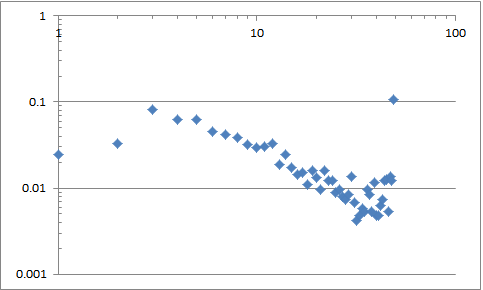
\includegraphics[width=4cm]{./figures/degrees_lastfm_users.png}} 
  &
  \subfloat[Twitter
  Users]{\label{fig:degrees_twitter_users}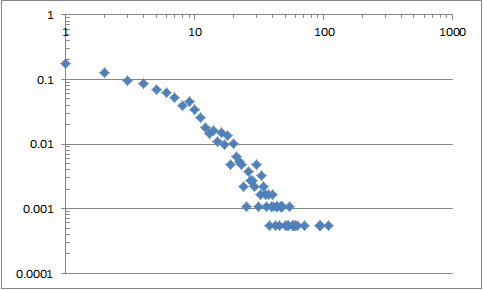
\includegraphics[width=4cm]{./figures/degrees_twitter_users.png}} 
  &
  \subfloat[Audioscrobbler
  Users]{\label{fig:degrees_audioscrobbler_users}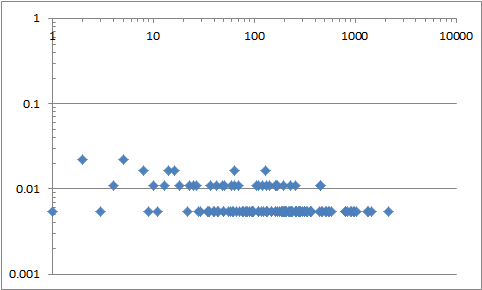
\includegraphics[width=4cm]{./figures/degrees_audioscrobbler_users.png}}
  \\
  \end{tabular}
  \begin{tabular}{cc} 
  \subfloat[Movielens
  Users]{\label{fig:degrees_movielens_users}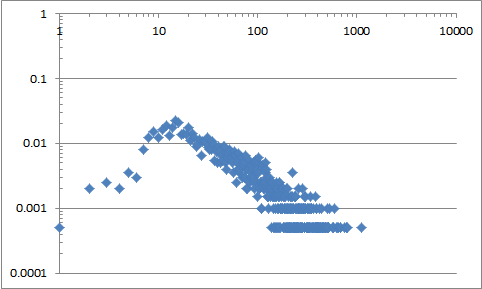
\includegraphics[width=4cm]{./figures/degrees_movielens_users.png}}
  &
  \subfloat[Delicious
  Users]{\label{fig:degrees_delicious_users}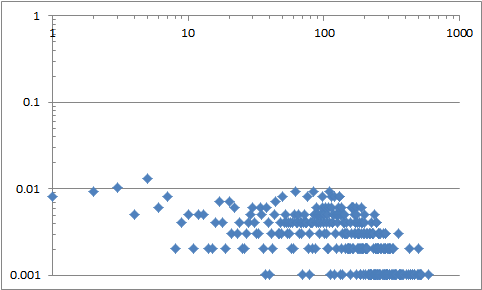
\includegraphics[width=4cm]{./figures/degrees_delicious_users.png}}
  \\ 
  \end{tabular}
  \caption{Degree distributions of users for the real world data sets}
  \label{fig:degrees_users}
\end{figure}

One of the most important structural property of networks is the degree
distribution. In the case of bipartite networks and users-objects networks
specifically, distributions of both types of nodes are considered.
According to previous studies, users degree generally follow an exponential
distribution
\citep{latapy2008basic}, or stretched exponential \citep{laherrere1998stretched}
at most, as shown in \citet{shang10empirical} or \citet{grujic2009mixing}. On
the other side, according to the same papers, the degree distribution of objects
follow a heavy tail distribution (power law or similar). This has important
consequences on the structure of the projected network and also on the process
of clustering the user nodes. Other bipartite networks like author-paper or
actor-movie doesn't exhibit this property as there is an inherent constraint on
how many authors can write a paper or how many actors can play in a movie.

\begin{figure}[t] \centering
  \begin{tabular}{ccc} 
  \subfloat[Last.fm
  Tags]{\label{fig:degrees_lastfm_objects}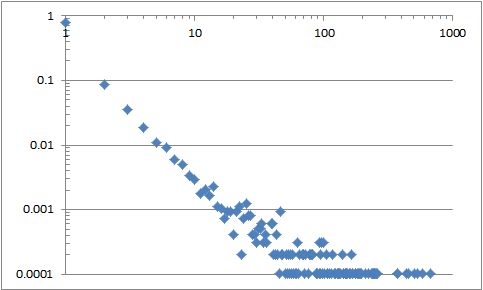
\includegraphics[width=4cm]{./figures/degrees_lastfm_objects.png}}
  & 
  \subfloat[Twitter
  Domains]{\label{fig:degrees_twitter_objects}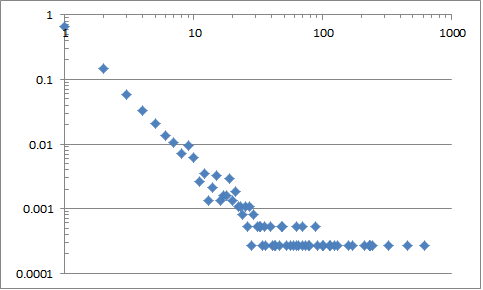
\includegraphics[width=4cm]{./figures/degrees_twitter_objects.png}}
  &
  \subfloat[Audioscrobbler
  Artists]{\label{fig:degrees_audioscrobbler_objects}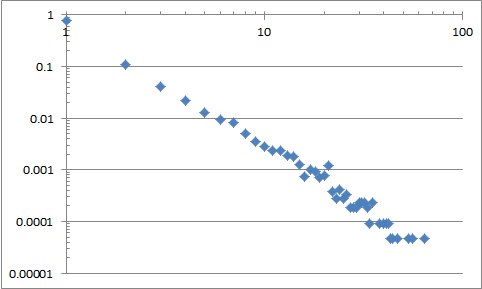
\includegraphics[width=4cm]{./figures/degrees_audioscrobbler_objects.png}}
  \\
  \end{tabular}
  \begin{tabular}{cc} 
  \subfloat[Movielens
  Movies]{\label{fig:degrees_movielens_objects}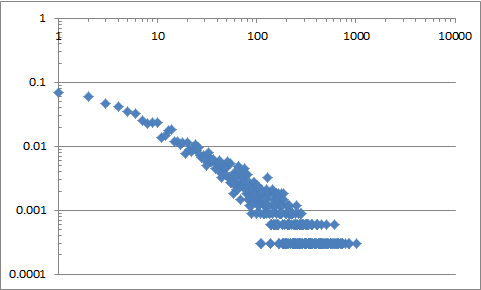
\includegraphics[width=4cm]{./figures/degrees_movielens_objects.png}}
  &
  \subfloat[Delicious
  Tags]{\label{fig:degrees_delicious_objects}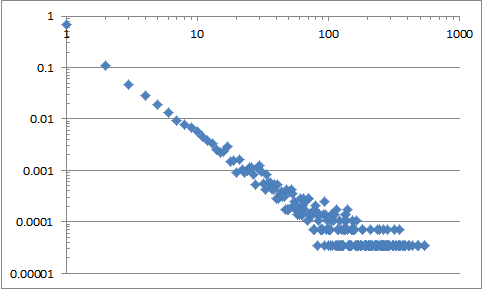
\includegraphics[width=4cm]{./figures/degrees_delicious_objects.png}}
  \\
  \end{tabular}
  \caption{Degree distributions of objects for the real world data sets}
  \label{fig:degrees_objects}
\end{figure}

Degree distributions of our sample user-object networks are shown in figures
\ref{fig:degrees_users} and \ref{fig:degrees_objects}. In order to find the
closest model that fits the data, for each such empirical distribution we
evaluate the goodness of fit of multiple distribution models by using
loglikelihood ratios as described in \citet{clauset2009power}. The results, for
both users and objects, are presented in Table \ref{tab:dist_bestfit}.

\begin{table}[!h] \centering
\begin{tabular}{ l | c c | c c }
\multirow{2}{*}{Data} & \multicolumn{2}{c}{Users} & \multicolumn{2}{c}{Objects}
\\
\cline{2-5}
& Best fit & Parameters & Best fit & Parameters \\
\hline
Last.fm & exponential & $\lambda = 0.054$ & lognormal & $\mu = -33.18$ \\
Twitter & lognormal & $\mu = 1.41$ & powerlaw & $\alpha = 2.05$ \\
Audioscrobbler & exponential & $\lambda = 0.0046$ & lognormal & $\mu = -2.75$ \\
Movielens & lognormal & $\mu = 4.07$ & lognormal & $\mu = 2.84$ \\
Delicious & exponential & $\lambda = 0.0081$ & lognormal & $\mu = -9.34$ \\
\hline
\end{tabular}
\caption{Best fit for degree distributions, users and objects.}
\label{tab:dist_bestfit}
\end{table}

While degree distribution for users (active nodes) don't expose a heavy tail in
most cases, the degree  distribution for objects (passive nodes) fits to one of
the distribution models with a tail that is not exponentially bounded (i.e.
power law or lognormal). Due to the number of high degree values (highly popular
objects), a heavy tail with heterogeneous distribution of degrees has a
significant impact on the structure of the projected network and consequently on
the community structure.

\paragraph{Clustering and impact of highly popular objects}

Clustering or community structure \citep{newman2004finding} is another property
of user-object or consumer-product networks. Users or consumers tend to cluster
together based on the common interests represented by the common objects they
are interacting with \citep{huang2007analyzing}. This property sits at the core
of the recommender systems based on collaborative filtering
\citep{breese1998empirical}. However, detecting communities in bipartite
networks is somehow challenging with few optimized options available at large
scale \citep{fortunato2010community}.

A popular approach is to project the bipartite network on one of its node sets
($U$ or $O$) and apply the community detection algorithm on the projected
network. As seen above, the projection of user-object networks where degrees of
objects follow a power law distribution is causing edge inflation in the
resulted network by increasing significantly the density of edges (hundreds of
times more). This affects the clustering in two ways. First, it `dilutes` the
clusters and decreases the quality of the community structure because of a
highly homogeneous distribution of edges among the nodes
\citep{fortunato2010community}. Second, it causes a drop in performance of
community detection algorithms, most of them optimized for sparse networks. For
example, popular algorithms like \citet{clauset2004finding},
\citet{raghavan2007near} or \citet{blondel2008fast} scale extremely well on
sparse data but are much less efficient when networks are very dense (number of
links $m$ are much larger than number of nodes $n$).

In our case, due to the heavy-tail distributions of objects, user-projections of
all five real-world networks are extremely dense ranging from 26\% to 89\%
(Table \ref{tab:datasets_prj}) causing difficulties such as those described
above. For example, by looking at the most popular objects in Table
\ref{tab:topdegrees} one can see that the highest degree node in each case
connects together more than a third of users and in some cases even 50\%.

\begin{table}[!h] \centering
\begin{tabular}{cc}
 
\subfloat[Last.fm user-tag] {
\begin{tabular}{ l | c c c c }
Tag & Degree & Users \\
\hline
rock & 673 & 35.5\% \\
pop & 585 & 30.9\% \\
alternative & 532 & 28.1\% \\
\end{tabular}
}

\subfloat[Twitter user-domain] {
\begin{tabular}{ l | c c c c }
Domain & Degree & Users \\
\hline
twitter.com & 611 & 33.2\% \\
facebook.com & 451 & 24.5\% \\
youtube.com & 324 & 17.6\% \\
\end{tabular}
}
\end{tabular}

\begin{tabular}{cc}
\subfloat[Audioscrobbler user-artist] {
\begin{tabular}{ l | c c c c }
Artist & Degree & Users \\
\hline
Radiohead & 65 & 35.5\% \\
Coldplay & 56 & 30.6\% \\
The Beatles & 53 & 28.9\% \\
\end{tabular}
}

\subfloat[Movielens user-movie] {
\begin{tabular}{ l | c c c c }
Movie & Degree & Users \\
\hline
American Beauty & 1009 & 50.4\% \\
Star Wars IV & 855 & 42.7\% \\
Star Wars V & 841 & 42\% \\
\end{tabular}
}
\end{tabular}

\begin{tabular}{c}
\subfloat[Delicious user-tag] {
\begin{tabular}{ l | c c c c }
Tag & Degree & Users \\
\hline
design & 546 & 56.1\% \\
video & 543 & 55.8\% \\
google & 489 & 50.2\% \\
\end{tabular}
}

\end{tabular}
\caption{Top objects by degree with percentage of users each object connects.}
\label{tab:topdegrees}
\end{table}

On the other side, these highly popular objects contain very little or very high
level information about the particularities of the adjacent users and are not
very meaningful for grouping users together. 

For example, while Last.fm tags like 'rock', 'pop' or 'alternative' might
contain some high level information on the users groups, it doesn't bring
specific information about these. In the meantime, unpopular (degree 5) tags
like 'symphonic rock', 'david bowie' or 'true norwegian black metal' are showing
narrow user interests. Also, highly popular tweeted domains like 'twitter.com'
or 'facebook.com' are very broad with little clustering information, while
unpopular domains like 'radioamerica.org' or 'seacoastonline.com' are much more
specific. This is in line with \citet{shang10empirical} who found that users
connected to unpopular objects have much higher similarity to each other than
the average. Therefore unpopular objects are considered a better indicator for
users common interests than popular ones.

One simple way to handle this problem is to remove the objects from the long
tail of the degree distribution (highest degree objects), but this will result
in loss of information overall, especially in cases when these objects are
reinforced frequently by some users. The proposed method in section
\ref{sec:tfidf} will address this issue by trying to find a balance between how
often an user interacts with an object and how popular an object is in the
network.
